\section{Parallel algorithms for $k$-Tree and network scan statistics}
\label{sec:applications}

We now describe parallel algorithms for our two problems by reducing them to
instances of the $k$-MLD problem. We discuss here how the corresponding polynomials
and DAGs are constructed implicitly and evaluated in the subroutine \parcircuit{};
the main Algorithm \parmaxwt{} remains unchanged. We recall the notation from Section \ref{sec:prelim}.

\subsection{$k$-Tree}
\label{sec:apps-trees}
For brevity, we describe the algorithm for the case where $H$ is a path; the
case of $H$ being a tree has a similar structure. We first describe how this is
reduced to a $k$-MLD instance (this follows from \cite{koutis:icalp08, williams2009finding}). Given a graph $G(V, E)$, let $x_v$ denote a variable associated with each node $v\in V$.
We define poynomials $P_v(i)$ for all $v\in V$, $i\leq k$ in the following manner.

\begin{itemize}
\item
$P_v(1) = x_v$ for all $v\in V$
\item
For $i>1$,
$P_v(i) = \sum_{i'<i} \sum_{u\in\nbr(v)} P_u(i')P_v(i-i')$
\item
Define the polynomial $P(x_1,\ldots,x_n) = \sum_v P_v(k)$
\end{itemize}

It can be verified that the graph $G$ has a path of length $k$ if and only if the
polynomial $P(x_1,\ldots,x_n)$ has a multilinear term. Algorithm \parcircuit\textsc{Path}
runs on the graph $G(V, E)$ directly (instead of a DAG), and this is partitioned
into subsets $V_1,\ldots, V_{N_1}$. Let $V_p$ denote the partition assigned to processor $p$.
The algorithm maintains variables $\val(i, j, q)$ for each node $i$, each $j\leq k$, and
iteration $q$ within the $t$th phase.

\begin{algorithm}{}
\small
\caption{\parcircuit\textsc{Path}{$(G(V, E), k, \mathbf{v}, t, N_2, N_1, \mathcal{P})$}}
\label{alg:parEvaluatepath} 
\begin{algorithmic}[1]
\STATE \textbf{Input:} Graph $G(V, E)$, parameter $k$, node levels $\mathcal{L}$, 
random assignment $\mathbf{v}$, phase number $t$, number of iterations within phase $N_2$,
number of partitions $N_1$, and partitioning $\mathcal{P}$
\STATE

\STATE \textbf{for} each processor $p$ in parallel do
\STATE \quad \textbf{for} $s=1$ to $k$ \textbf{do}
\STATE \quad \quad \textbf{for} each node $i\in V_p$ \textbf{do}
\STATE \quad \quad \quad \textbf{if} $s=1$ $ \val(i, 1, q) = 1 + (-1)^{v_i^T \cdot q_{\text{bin}}}$
\STATE \quad \quad \quad \textbf{if} $s>1$ compute $\val(i, s, q) =$
\STATE \quad \quad \quad \quad \quad $\sum_{s'<s} \sum_{i'\in\nbr(i)} \val(i', s', q)\val(i, s-s', q)$
\STATE \quad \quad \quad \textbf{Send result to neighbors in other processors}
\STATE \quad \quad \quad \textbf{for} $i' \in \nbr(i) \setminus V^{p}$ \textbf{do}
\STATE \quad \quad \quad \quad \textbf{Send} $\langle i, \val(i, s, q)\rangle$
\STATE \textbf{return} $\sum_q \val($root$(G), q)$
\end{algorithmic}
\end{algorithm}

\iffalse
\comment{move the rest of this to the supplementary}

\begin{figure}[h]
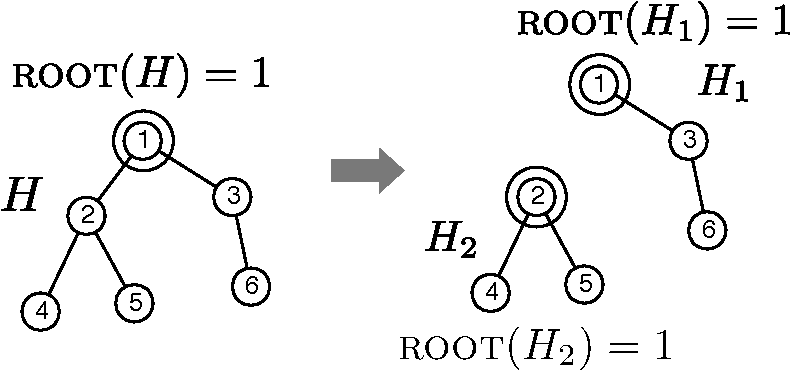
\includegraphics[width=0.4\textwidth]{img/trees.pdf}
\caption{
\small
Tree $H$ with $\myroot(H)=1$. It is decomposed into trees $H_1$ and $H_2$ by
removing the edge $(1, 2)$. $\myroot(H_1)=1$ and $\myroot(H_2)=2$.
%\vspace{-0.2in}
}
\label{fig:trees}
\end{figure}
Next, we consider the case where $H$ is a tree. We consider the tree to be rooted,
and let $\myroot(H)$ be the root node, selected arbitrarily. We consider a hierarchical
structure among subtrees of $H$ in the following manner: consider any node $u\in\nbr(\myroot(H))$.
Let $H_1$ and $H_2$ denote the subtrees obtained upon deleting the edge $(u, \myroot(H))$,
with $\myroot(H)\in H_1$ and $u\in H_2$. We set $\myroot(H_1)=\myroot(H)$ and $\myroot(H_2)=u$.
This process is illustrated i Figure \ref{fig:trees}.
The subtrees $H_1$ and $H_2$ are further partitioned in a recursive manner, till
all trees have a single node. For an intermediate tree $H'$ in this process,
let $\textsc{child}_1(H')$ and $\textsc{child}_2(H')$ denote the two child trees
resulting from the tree $H'$. Let $\textsc{parent}(H')=H''$ be the tree such that
either $\textsc{child}_1(H'')= H'$ or $\textsc{child}_2(H'') = H'$.
We define the polynomials $P_v(H')$, which will correspond to all layouts (not necessarily
isomorphisms) of $H'$ with $\myroot(H')=v$, in the following manner:
\begin{itemize}
\item
If $H'$ consists of a single node, $P_v(H') = x_v$
\item
Else, 
$P_v(H') = \sum_{u\in\nbr(v)} P_v(H'_1)P_u(H'_2)$, where
$H'_1$ and $H'_2$ denote $\textsc{child}_1(H')$ and $\textsc{child}_2(H')$, respectively.
\item
Finally, we have
$P(x_1,\ldots, x_n)= \sum_v P_v(H)$
\end{itemize}

More generally, we consider a weighted version of the problem, where the goal is to
find an embedding of the maximum weight. 
\fi 

\subsection{Scan Statistics}
\label{sec:apps-scanstat}
%For concreteness, we now show how to implement a sequential algorithm for Problem \ref{prob:macs} based on the Multilinear Detection technique. We start by describing how to recursively construct and evaluate a circuit for this problem.
Let $W(V) = \sum_v{w(v)}$ be the total weight of the nodes in $G$. For each node $v$, we define a variable $x_v$, and we construct a polynomial over the set of variables $\{x_v: v \in V\}$. Every term---i.e., monomial---in this polynomial will represent a connected subgraph of size at most $k$ and weight at most $W(V)$.
For $i \leq K$ and $j \leq W(V)$, let $P_v(i,j)$ be the polynomial corresponding to a subgraph (1) containing node $v$, (2) of size $i$, and (3) total weight
$j$. The following recurrence relations describe how the polynomials $P_v(i, j)$ are computed:
\begin{itemize}
\item
$P_v(1, j) = x_v$ for all $v \in V$, $j = w(v)$
\item
For $v \in V$, $i = 2$ to $k$, $j = 0$ to $r$, 
$P_v(i,j) = \sum_{u \in \nbr(v)} \sum_{i' = 1}^{i-1}\sum_{j'=0}^j (P_v(i', j') \cdot P_u(i-i', j - j'))$
\item
$P(i,j) = \sum_v P_v(i,j)$ for $i \in K$, $j \in R$
\end{itemize}
Algorithm \ref{alg:parEvaluateScanStat} maintains variables $\val(i, j, \ell, q)$ for every node $i$, $j\leq k$, $\ell \leq W(V)$, and iteration $q$ within phase $t$. It can be verified that the input graph $G$ has a connected subgraph $S$ of weight $W(S)$ if and only if the corresponding polynomial $P(i, j)$ has a multilinear term.

%\noindent
%\subsubsection{High level idea of \textsc{MLD-ScanStat} (Algorithm \ref{alg:mld-scanstat})}
%After selecting random vectors from $\mathbb{Z}_2^k$ for each circuit input (line 6), 
%we compute the polynomial by performing $2^k$ evaluations of the circuit (lines 8--24). 
%The $t$-{th} evaluation gives us the value of the $(t + 1)$-th row in the matrix 
%representation, as discussed in Section \ref{sec:prelim}. We evaluate the circuit following its recursive definition. First, we initialize the circuit inputs in the base case (lines 11--13) 
%to be the $t$-th eigenvalue of their respective matrix representation, which is computed 
%as $1 + (-1)^{x_v^T\cdot t_{\text{bin}}}$, where $x_v$ is the random vector assigned to node 
%$i$ and $t_{\text{bin}}$ is the $k$-bit binary representation of $t$. 
%Then, for each $i \leq k$, we evaluate the circuit by aggregating values from nodes of the form $P_v(i')$, for some $i' < i$, which have already been computed in 
%a previous iteration of the \textbf{for} loop. 
%We show an example of this algorithm in Figure \ref{fig:algorithm-example}.

%%%\begin{figure*}[!htbp]
%%%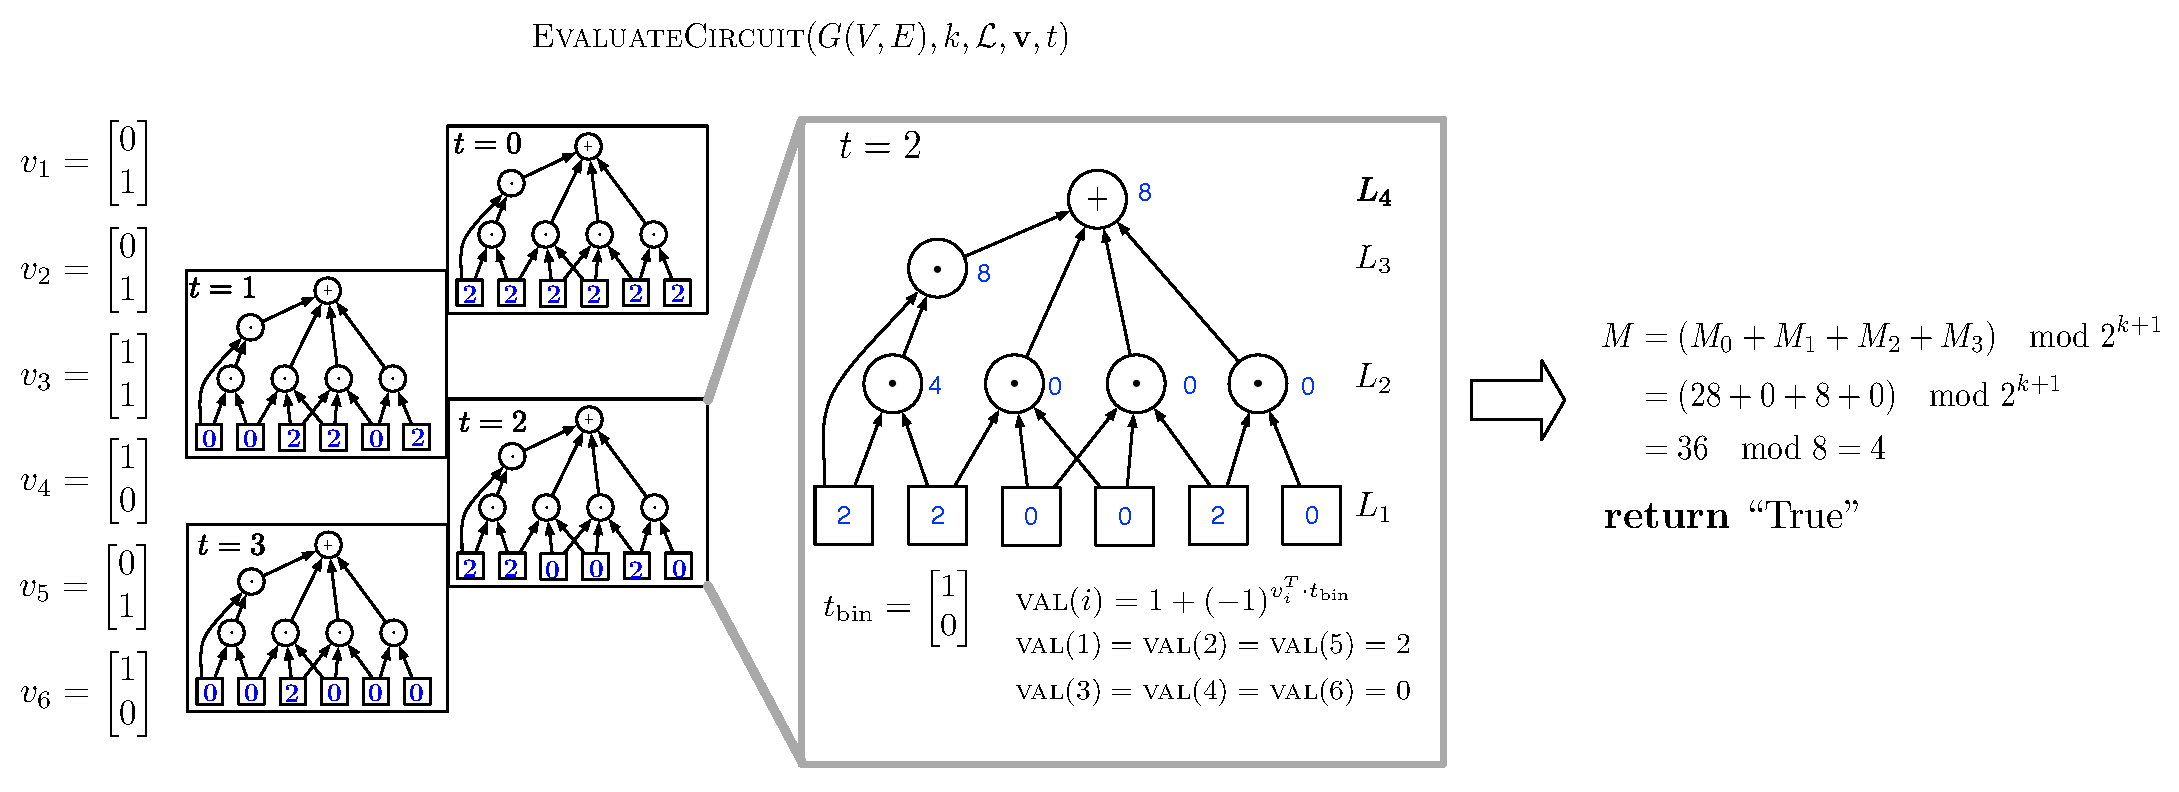
\includegraphics[width=\textwidth]{img/algorithm-example-v2_fixed.pdf}
%%%\caption{
%%%\small
%%%Example of the sequential algorithm \maxwt{}. The input is the circuit $G(V,E)$ from
%%%Figure \ref{fig:dag} with 12 nodes on four levels, $L_1$, $L_2$, $L_3$ and $L_4$, as shown.
%%%The algorithm picks the vectors $v_1,\ldots,v_6$ from $\mathbb{Z}_2^2$, as shown in
%%%the left of the figure. Since $k=2$, there are $2^k=4$ iterations, corresponding to
%%%$t=0,\ldots,3$. The values of $\val(v)=1+(-1)^{v^Tt_{bin}}$ for the $t$th iteration
%%%are shown in blue as the input values. The outputs of the circuit are $M_0, \ldots, M_3$,
%%%with values as shown in the right of the figure. For these choices of the $v_i$'s, the
%%%computed value $M\neq 0 (\text{mod } 2^{k+1})$, which implies the existence of a
%%%multilinear term with $k$ variables. This is true because the term $x_5x_6$ in the
%%%polynomial is indeed multilinear.
%%%%---IDs are in red---$k=2$, and 3 levels. Nodes 1 through 6 are the first level---i.e., the circuit inputs. Nodes 7 through 10 are the second level, all with multiplication operation ($op(i) = \cdot$). The last level only contains the root of the circuit, with addition operation. First, the algorithm generates random vectors $v_i$ for the circuit inputs (bottom left). Then, the circuit is evaluated $2^k$ times by calling procedure \algcircuit{} (center). We show the evaluation for iteration $t=2$. First, we compute the inputs to the circuit as $1 + (-1)^{v_i^T\cdot t_{\text{bin}}}$---this will always be either 2 or 0. From there, we can evaluate the circuit by levels. Finally, back in \maxwt{}, we aggregate the value at root$(G)$ over all the iterations (right). In this case, the polynomial evaluates to $0$, so we return ``False".
%%%%\vspace{-0.2in}
%%%}
%%%\label{fig:algorithm-example}
%%%\end{figure*}

%\begin{algorithm}{}
%\small
%\caption{\maxwt{}$(G(V, E), k$.}
%\label{alg:multilinear-detect}
%\begin{algorithmic}[1]
%\STATE \textbf{Input}: Graph $G(V, E)$, parameter $k$
%\STATE\textbf{Output}: ``True" if circuit evaluation is non-zero. ``False" otherwise.
%\STATE \textbf{Initialize circuit inputs}
%\STATE \textbf{for} node $i \in L_1$ \textbf{do}
%\STATE \quad Let $v_i$ be a random vector from $\mathbb{Z}_{2}^k$
%\STATE \textbf{Initialize the polynomial}
%\STATE Let $M = \bar 0$
%\STATE \textbf{Evaluate circuit for each row of matrix representation}
%\STATE \textbf{for} $t = 0$ to $2^{k-1}$ \textbf{do}
%\STATE \quad $M_t = \algcircuit(G(V, E), k, \mathcal{L}, \mathbf{v}, t)$
%\STATE $M = \sum_{t=0}^{2^{k-1}} M_t \mod 2^{k+1}$
%\STATE \textbf{return} $M \neq 0$
%\STATE
%\STATE \textbf{procedure} \algcircuit{$(G(V, E), k, \mathcal{L}, \mathbf{v}, t)$}
%\STATE \textbf{Input}: Circuit $G(V, E)$, parameter $k$, node levels $\mathcal{L}$, random assigment $\mathbf{v}$, and iteration number $t$
%\STATE\textbf{Output}: Value at root node of $G(V,E)$
%\STATE \textbf{Initialize circuit inputs}
%\STATE \textbf{for} node $i \in L_1$ \textbf{do}
%\STATE \quad $ \val(i) = 1 + (-1)^{v_i^T \cdot t_{\text{bin}}}$
%
%\STATE \textbf{Evaluate the circuit by levels}
%\STATE \textbf{for} $s=2$ to $|\mathcal{L}|$ \textbf{do}
%\STATE \quad \textbf{for} $i \in L_s$ \textbf{do}
%\STATE \qquad \textbf{if} $\op(i) = +$ \textbf{then}
%\STATE \qquad \quad $\val(i) = 0$
%\STATE \qquad \quad \textbf{for} $j \in \pred(i)$ \textbf{do}
%\STATE \qquad \qquad $\val(i) = \val(i) + \val(j)$
%\STATE \qquad \textbf{else} 
%\STATE \qquad \quad $\val(i) = 1$
%\STATE \qquad \quad \textbf{for} $j \in \pred(i)$ \textbf{do}
%\STATE \qquad \qquad $\val(i) = \val(i) \cdot \val(j)$
%
%\STATE \textbf{return} $\val($root$(G))$
%\end{algorithmic}
%\end{algorithm}

%\begin{algorithm}{}
%\small
%\caption{\small \textsc{MLD-ScanStat}$(G(V, E), \mathbf{w}, k, \epsilon, r)$.}
%\label{alg:mld-scanstat}
%\begin{algorithmic}[1]
%\STATE \textbf{Input}: Instance $(G(V, E), \mathbf{w})$ and parameters $k, \epsilon, r$
%\STATE\textbf{Output}: "True" if $G$ has a subgraph $S$ with size $i \leq k$ and weight $j \leq r$
%\STATE Let $K=\{1,\ldots,k\}, R=\{0, \ldots, r\}$
%\STATE \textbf{Initialize the polynomial}
%\STATE $P(i, j) = \bar{0}$ for $i \in K$, $j \in R$
%\STATE For each node $v$, pick a random vector $x_v \in Q[\mathbb{Z}_{2}^k]$
%\STATE \textbf{Evaluate the circuit for each row of matrix representation}
%\STATE \textbf{for} $t = 0$ to $2^{k-1}$
%\STATE \quad $P_v(i, j) = \bar{0}$ for $i \in K$, $j \in R$
%\STATE \quad \textbf{Initialize circuit inputs}
%\STATE \quad \textbf{for} $v \in V$ \textbf{do}
%\STATE \quad \quad $P_v(1, w(v)) = 1 + (-1)^{x_v^T \cdot t_{\text{bin}}}$
%\STATE \quad \textbf{Evaluate circuit recursively}
%\STATE \quad \textbf{for} $v \in V$, $i = 2$ to $k$, $j = 0$ to $r$ \textbf{do}
%\STATE \qquad $P_v(i,j) = \sum_{u \in \nbr(v)} \sum_{i' = 1}^{i-1}\sum_{j'=0}^j (P_v(i', j') \cdot P_u(i-i', j - j'))$ 
%\STATE
%\STATE \textbf{return} $P \neq \bar 0$
%\end{algorithmic}
%\end{algorithm}

\begin{algorithm}{}
\small
\caption{\parcircuit\textsc{ScanStat}{$(G(V, E), k, \mathbf{v}, t, N_2, N_1, \mathcal{P})$}}
\label{alg:parEvaluateScanStat} 
\begin{algorithmic}[1]
\STATE \textbf{Input:} Graph $G(V, E)$, parameter $k$, node levels $\mathcal{L}$, 
random assignment $\mathbf{v}$, phase number $t$, number of iterations within phase $N_2$,
number of partitions $N_1$, and partitioning $\mathcal{P}$
\STATE
\STATE \textbf{for} each processor $p$ in parallel do
\STATE $\val(i, s, \ell, q) = 0$ for $i\in V, s \leq k, \ell \leq W(V), q$
\STATE \quad \textbf{for} $s=1$ to $k$ \textbf{do}
\STATE \quad \quad \textbf{for} each node $i\in V_p$ \textbf{do}
\STATE \quad \quad \quad \textbf{if} $s=1$ $ \val(i, 1, w(v), q) = 1 + (-1)^{v_i^T \cdot q_{\text{bin}}}$
\STATE \quad \quad \quad \textbf{if} $s>1$ compute $\val(i, s, \ell, q) =$
\STATE \quad \quad \quad \quad \quad $\sum_{\ell'=0}^\ell \sum_{s'<s} \sum_{i'\in\nbr(i)} \val(i', s', \ell', q)\val(i, s-s', \ell - \ell', q)$
\STATE \quad \quad \quad \textbf{Send result to neighbors in other processors}
\STATE \quad \quad \quad \textbf{for} $i' \in \nbr(i) \setminus V^{p}$ \textbf{do}
\STATE \quad \quad \quad \quad \textbf{Send} $\langle i, \val(i, s, \ell, q)\rangle$
\STATE \textbf{return} $\sum_q \val($root$(G), q)$
\end{algorithmic}
\end{algorithm}